\section{Puppet}
Puppet là một framework mã nguồn mở và là công cụ để quản lý cấu hình của hệ thống máy tính. Trong phần này, chúng ta sẽ tìm hiểu tổng quan về Puppet: cách thức nó hoạt động, cách nó quản lý cấu hình của hệ thống máy chủ, lý do puppet có thể chạy trên nhiều nền tảng khác nhau. Tiếp đó, chúng ta sẽ tìm hiểu kiến trúc của Puppet, cách Puppet thu thập và quản lý các gói dữ liệu cấu hình.

\subsection{Tổng quan}
Puppet là một công cụ quản lý cấu hình mã nguồn mở viết bằng Ruby, được sử dụng để quản lý cấu hình máy chủ và tự động hóa hệ thống trong các trung tâm dữ liệu của Google, Twitter, thị trường chứng khoán New York, và nhiều doanh nghiệp lớn khác. Puppet được phát triển đầu tiên bởi Puppet Labs, và hiện tại Puppet Labs cũng là người duy trì chính của dự án này. Puppet được dùng để quản lý có khi chỉ vài máy chủ nhưng cũng có khi lên tới 50.000 máy chủ, cùng với đó là đội quản trị hệ thống từ một người tới hàng trăm người.

Puppet là một công cụ để quản lý cấu hình và bảo trì hệ thống máy tính; ngôn ngữ cấu hình của nó rất đơn giản. Chúng ta chỉ cần chỉ cho Puppet thấy chúng ta muốn cấu hình máy tính của chúng ta như thế nào, nó sẽ thực hiện đúng những gì chúng ta muốn. Khi hệ thống có sự thay đổi chẳng hạn như một phiên bản cập nhật của gói phần mềm, thêm người dùng mới hay một cấu hình nào đó thay đổi, Puppet tự động cập nhật tất cả các máy chủ trong hệ thống đúng như cấu hình chúng ta muốn.

\begin{figure}[htb]
    \begin{center}
    \fbox{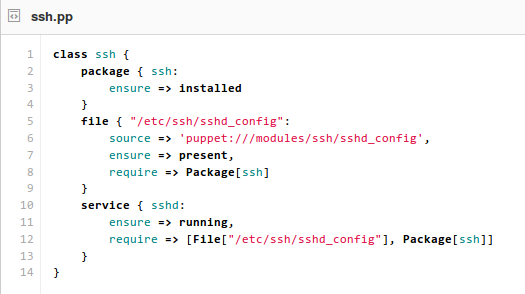
\includegraphics[width=0.9\textwidth]{images/puppet_ssh_pp.png}}
    \end{center}
    \caption{Ví dụ về ngôn ngữ cấu hình của Puppet}
    \label{fig:puppet_ssh_pp}
\end{figure}

Như hình vẽ trên, Puppet đảm bảo rằng gói phần mềm \textbf{\textit{ssh}} được cài đặt và file cấu hình dịch vụ SSH \footnote{Secure Shell: \url{https://en.wikipedia.org/wiki/Secure_Shell}} \textbf{\textit{/etc/ssh/sshd\_config}} của tất cả các máy chủ trong hệ thống mà Puppet quản lý đều có cùng nội dung mới file đã định trước; thêm vào đó, Puppet đảm bảo việc dịch vụ này luôn được chạy giúp người quản trị hệ thống có thể can thiệp thủ công khi cần thiết.

\subsection{Kiến trúc hệ thống}

Puppet được xây dựng với hai chế độ làm việc:

\begin{itemize}
\item \textbf{Chế độ client/server} Có một máy chủ trung tâm với một dịch vụ chạy nền kết nối đến các "agents" chạy độc lập trên các máy trạm.

\item \textbf{Chế độ serverless} Chỉ có một tiến trình duy nhất thực hiện tất cả các công việc.
\end{itemize}

Để đảm bảo tính nhất quán giữa các chế độ, Puppet luôn có sự minh bạch trong các liên kết nội bộ của bản thân nó. Do đó, hai chế độ này sử dụng cùng một đường dẫn như nhau cho dù chúng có giao tiếp với nhau qua mạng hay không. Mỗi lệnh được thực thi cho dù lấy cấu hình từ bản nó hay một máy khác ở xa trong mạng thì chúng đều có một cách thực hiện như nhau. Tuy nhiên cũng phải lưu ý rằng, chế độ serverless là một phần trong trong mô hình client/server: tất cả các file cấu hình sẽ được đẩy xuống cho agents ở máy trạm xử lý, tại đây máy trạm chạy ở chế độ serverless sẽ làm việc trực tiếp với các tệp tin cấu hình và thực thi chúng. Phần này sẽ chỉ tập trung vào chế độ client/server bởi vì nó dễ hiểu hơn với các thành phân riêng biệt, nhưng hãy luôn nhớ rằng tất cả đều chạy ở chế độ serverless.

Một trong những lựa chọn ngay từ đầu trong kiến trúc của Puppet là máy trạm không nên truy cập trực tiếp (raw access) vào các module, thay vào đó, chúng lấy các cấu hình đã được chuẩn bị sẵn từ trước. Việc này cung cấp nhiều lợi ích:

\begin{itemize}
\item \textbf{Thứ nhất}, chung ta thực hiện được việc tối thiểu quyền hạn cần thiết. Trong đó mỗi máy chủ chỉ biết chính xác những gì nó cần phải biết (nó nên được cấu hình như thế nào), nhưng nó không biết (và không quan tâm) những máy trạm khác được cấu hình như thế nào.

\item \textbf{Thứ hai}, chúng ta hoàn toàn có thể phân tách các quyền cần thiết để tạo ra một cấu hình (bao gồm cả quyền truy cập vào nơi lưu trữ dữ liệu trung tâm) mà nó sẽ được thực hiện dưới máy trạm.

\item \textbf{Thứ ba}, chúng ta có thể chạy các máy trạm trong chế độ ngắt kết nối với máy chủ trung tâm, nhưng các cấu hình đã có của Puppet sẽ vẫn luôn được áp dụng. Nghĩa là, cho dù máy chủ trung tâm (puppet-master) không còn hoạt động hoặc không có kết nối đến nó thì mỗi máy trạm vẫn có thể làm việc độc lập.

\end{itemize}

\begin{figure}[h!]
    \begin{center}
    \fbox{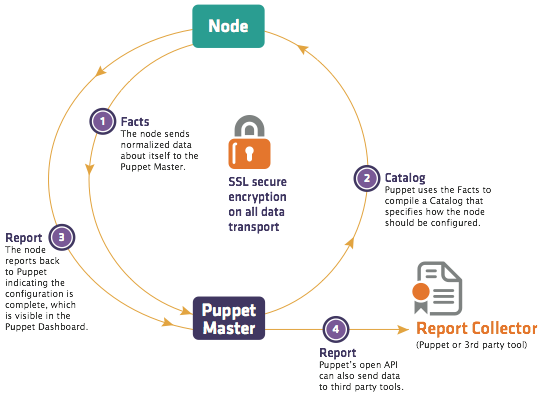
\includegraphics[width=0.9\textwidth]{images/puppet_dataflow.png}}
    \end{center}
    \caption{Biểu đồ luồng dữ liệu của Puppet}
    \label{fig:puppet_dataflow}
\end{figure}

Với sự lựa chọn này, quy trình làm việc trở nên tương đối đơn giản

\begin{itemize}
\item Tiến trình trên máy trạm (Puppet agent) thu thập các thông tin về hệ thống mà nó đang làm việc, sau đó chuyển các thông tin này tới máy chủ trung tâm (Puppet Master)

\item Tại máy chủ trung tâm, các thông tin đó cùng các module trên ổ đĩa cục bộ được biên dịch thành một cấu hình cho một máy chủ cụ thể và trả lại nó cho các tiến trình trên máy trạm.

\item Các tiến trình trên máy trạm áp dụng những cấu hình cục bộ này và nó chỉ ảnh hưởng tới riêng máy trạm đó. Sau đó, các tập tin báo cáo được tạo ra rồi đưa kết quả về máy chủ trung tâm.
\end{itemize}

Vì thế, các agent có quyền truy cập vào thông tin riêng trên hệ thống của mình, các cấu hình của bản thân nó, cũng như các báo cáo nó tạo ra. Máy chủ trung tâm có bản sao của tất cả các dữ liệu này, cùng với quyền truy cập toàn bộ các module, cũng như bất kỳ cơ sở dữ liệu và dịch vụ nào khác dùng để biên dịch các cấu hình cần thiết.

\begin{figure}[h!]
    \begin{center}
    \fbox{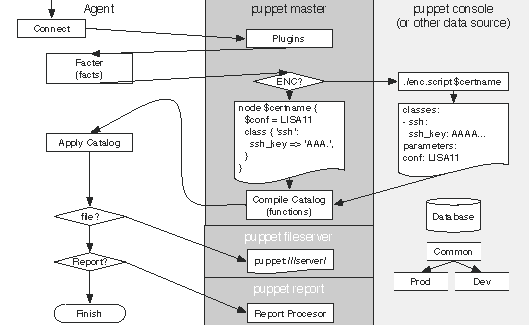
\includegraphics[width=0.9\textwidth]{images/puppet_timing_diagram.png}}
    \end{center}
    \caption{Luồng dữ liệu lưu chuyển \\ giữa các thành phần và tiến trình của Puppet}
    \label{fig:puppet_timing_diagram}
\end{figure}

Ngoài các thành phần ở trong quy trình làm việc này, có rất nhiều loại dữ liệu được Puppet sử dụng cho các giao tiếp nội bộ của nó. Các loại dữ liệu rất quan trọng, bởi vì chúng hoàn thực hiện tất cả các thông tin liên lạc, đồng thời chúng cũng cung cấp các giao diện công cộng cho những công cụ khác sử dụng hay làm việc với chúng.

\newpage
\clearpage
Các kiểu dữ liệu quan trọng nhất trong Puppet là:

\begin{itemize}
\item \textbf{Facts}: Thu thập các thông thin hệ thống trên mỗi máy trạm. Những thông tin này được dùng để biên dịch ra các cấu hình.

\item \textbf{Manifest}: Các tập tin chứa ngôn ngữ cấu hình Puppet, chúng thường được tổ chức thành các bộ sưu tập được gọi là module.

\item \textbf{Catalog}: Một đồ thị về các tài nguyên của máy chủ được quản lý và các rằng buộc giữa chúng.

\item \textbf{Report}: Tập hợp tất cả các sự kiện được tạo ra trong suốt quá trình tạo ra các Catalog.
\end{itemize}

Ngoài Facts, Manifests, Catalogs, and Reports, Puppet còn hỗ trợ các kiểu dữ liệu như các tệp tin, các chứng chỉ (được dùng trong việc xác thực) cùng nhiều kiểu dữ liệu khác.

\begin{figure}[h!]
    \begin{center}
    \fbox{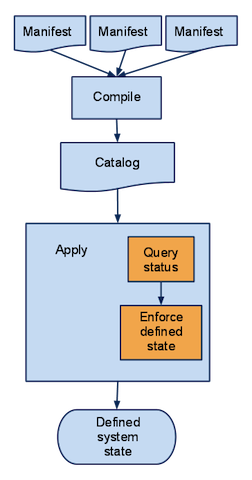
\includegraphics[scale=1.0]{images/puppet_manifest_to_defined_state_unified.png}}
    \end{center}
    \caption{Cách Puppet biên dịch và thực hiện một manifest\\ trong chế độ Serverless}
    \label{fig:puppet_manifest_to_defined_state_unified}
\end{figure}

\begin{figure}[h!]
    \begin{center}
    \fbox{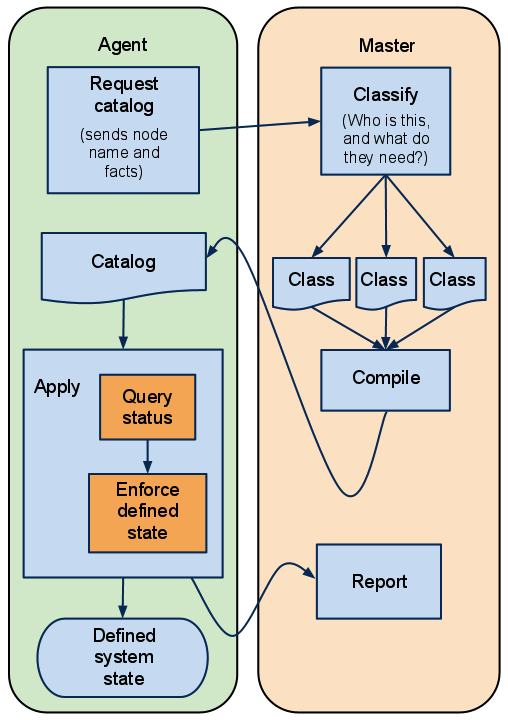
\includegraphics[width=0.85\textwidth]{images/puppet_manifest_to_defined_state_split.png}}
    \end{center}
    \caption{Cách Puppet biên dịch và thực hiện một manifest\\ trong chế độ Client-Server}
    \label{fig:puppet_manifest_to_defined_state_split}
\end{figure}

\clearpage
\subsection{Các thành phần chính}
Các thành phần chính của Puppet bao gồm: Agent, Facter, ENC, Compiler, Transaction, RAL và Reporting


\textbf{\large Agent}


Thành phần đầu tiên mà chúng ta tiếp xúc khi sử dụng Puppet là tiến trình agent. Trong các phiên bản trước của puppet, tiến trình này được tách riêng thành một tiến trình riêng biệt có tên là \textbf{\textit{puppetd}}, nhưng trong phiên bản 2.6 trở đi, chúng được tối giản hóa và bây giờ chúng được gọi bằng lệnh \textbf{\textit{puppet agent}}, tương tự như cách làm của Git\footnote{Một hệ thống quản lý mã nguồn phân tán \url{http://git-scm.com/}}. Các agent thực hiện rất ít các chức năng của riêng nó mà chủ yếu các công việc liên quan đến các cấu hình hay mã nguồn được thực hiện ở phía máy trạm như trong quy trình làm việc đã mô tả ở trên.


\textbf{\large Facter}


Thành phần tiếp theo sau agent là một công cụ bên ngoài gọi là \textbf{\textbf{facter}}, đó là một công cụ đơn giản được sử dụng để tìm kiếm và thu thập các thông tin về hệ thống nó đang chạy trên đó. Thông tin đó thường là hệ điều hành, địa chỉ IP, tên máy chủ, nhưng vì Facter là một công cụ có khả năng mở rộng nên rất nhiều các tổ chức thường thêm vào các plugin riêng họ để thu thập các thông tin khác mà họ cần. Các agent gửi những thông tin mà Facter đã thu thập được tới máy chủ trung tâm, nơi nó được tiếp quản và xử lý theo quy trình ở hình \ref{fig:puppet_dataflow}


\textbf{\large External Node Classifier}


Trên máy chủ trung tâm, thành phần đầu tiên chúng ta cần đề cập tới là External Node Classifier\footnote{Các lớp phân loại mở rộng} hay ENC. ENC chấp nhận tên máy trạm hoặc trả về các cấu trúc dữ liệu đơn giản có chứa các cấu hình cấp cao của máy chủ đó. ENC nói chung là một ứng dụng hay dịch vụ riêng biệt: điển hình là một vài sản phẩm mã nguồn mở như Puppet Dashboard hay Foreman; đôi khi nó được tích hợp vào hệ thống dữ liệu có sẵn chẳng hạn như máy chủ LDAP... Mục đích cơ bản của ENC là để xác định những gì mà các lớp chức năng thuộc về, kèm theo đó là những thông số cấu hình cho các lớp này. Ví dụ, một máy trạm có thể thuộc lớp \textbf{\textit{debian}} hay \textbf{\textit{webserver}} và chúng có tham số để báo rằng chúng ở trung tâm dữ liệu tại \textbf{\textit{atlanta}}

Lưu ý rằng như Puppet 2.7, ENC không phải là một thành phần bắt buộc, thay vào đó người dùng có thể trực tiếp chỉ định cấu hình tại mỗi nút của Puppet. ENC được hỗ trợ trong khoảng 2 năm sau khi Puppet ra đời, bởi vì những nhà phát triển nhận ra rằng các lớp về cơ bản là khác biệt với các việc cấu hình chúng. Và, nó sẽ có ý nghĩa hơn nhiều khi đưa những vấn đề này vào các công cụ riêng biệt thay vì mở rộng ngôn ngữ để hỗ trợ cả hai cơ sở này. ENC luôn luôn khuyến khích sử dụng, và tại một số nơi nó trở thành một thành phần cần thiết (lúc này Puppet sẽ xuất hiện với tư cách một công cụ hữu ích hơn là một gánh nặng).

Một khi máy chủ trung tâm nhận được thông tin phân loại theo lớp từ ENC và thông tin hệ thống từ facter (thông qua các agent), nó đóng gói tất cả các thông tin vào một đối tượng Node và chuyển nó vào các trình biên dịch (Compiler).


\textbf{\large Compiler}


Như đã đề cập ở trên, Puppet có một ngôn ngữ tùy chỉnh được xây dựng dành riêng cho việc cấu hình hệ thống. Trình biên dịch này bao gồm 3 khối: một bộ phân tích ngôn kiểu-Yacc\footnote{https://en.wikipedia.org/wiki/Yacc} đã được tùy chỉnh; một nhóm các lớp học sử dụng để tạo ra Cây cú pháp trừu tượng (Abstract Syntax Tree hay AST); sau cùng lớp biên dịch, nó xử lý các tương tác của tất cả các lớp, đồng thời cũng có chức năng như API và là một phần của hệ thống.


\textbf{\large Transaction}


Khi các Catalog đã được xây dựng thành công, nó được chuyển qua cho lớp Transaction. Trong một hệ thống mà máy trạm và máy chủ trung tâm được tách biệt, bộ phận này được chạy trên máy trạm, nó có nhiệm vụ kéo xuống các Catalog qua giao thức HTTP như Hình \ref{fig:puppet_timing_diagram}.

Lớp Transaction thực hiện một công việc tương đối đơn giản: tìm sự rằng buộc trong các mối quan hệ và đảm bảo các tài nguyên đấy được đồng bộ. Nó thực hiện một quá trình với 3 bước đơn giản: lấy trạng thái hiện tại của tài nguyên đó, so sánh nó với trạng thái mong muốn và thực hiện bất kì thay đổi cần thiết nào để sữa chữa sai lệnh.


\textbf{\large Resource Abstraction Layer}


Như đã biết, lớp Transcaction là rất quan trọng sự hoàn thành các công việc trong Puppet, nhưng thật ra, tất cả các công việc được thực sự thực hiện bởi lớp tài nguyên trừu tượng (Resource Abstraction Layer, viết tắt là RAL). Đây cũng là một trong các thành phần thú vị nhất của Puppet.

RAL là thành phần đầu tiên được tạo ra trong Puppet, hơn cả ngôn ngữ cấu hình, nó định nghĩa rõ ràng những gì con người có thể làm với nó. Công việc của RAL là xác định những gì là tài nguyên và cách các tài nguyên đó có thể thực hiện công việc của nó trên hệ thống. Sau đó ngôn ngữ Puppet được cụ thể hóa thành các mô hình bằng RAL. Bởi vì điều này nên nó là thành phần quan trọng nhất trong hệ thống, và khó khăn nhất để thay đổi. Có rất nhiều điều những nhà phát triển muốn khắc phục trong RAL, và họ đã thực hiện rất nhiều cải tiến quan trọng đối với nó trong nhiều năm qua (quan trọng nhất là việc bổ sung các Providers ), nhưng vẫn có rất nhiều việc phải làm với RAL trong dài hạn.

Như đã nói, lớp Transaction không thực sự ảnh hưởng  trực tiếp đến hệ thống, mà nó dựa vào RAL để làm việc đó. Trong thực tế, providers là thành phần duy nhất của Puppet mà thực sự tác động vào hệ thống. Nếu lớp Transaction yêu cầu nội dung của một tập tin thì lớp Providers tìm kiếm và thu thập nó; nếu lớp Transaction xác định rằng nội dung của một tập tin nên được thay đổi thì lớp Providers sẽ thay đổi nó. Tuy nhiên phải lưu ý rằng, bản thân lớp Providers không bao giờ có quyền quyết định ảnh hưởng đến hệ thống mà chính lớp Transaction mới có quyền này, lớp Providers chỉ là người thực hiện công việc. Điều này cho phép các lớp Transaction kiểm soát hoàn toàn mà không yêu cầu phải hiểu bất cứ điều gì về các tập tin, người dùng, hoặc các gói. Sự phân chia rõ ràng này cho phép Puppet có sự mô phỏng đầy đủ nơi mà chúng ta có thể đảm bảo phần lớn hệ thống không bị ảnh hưởng.


\textbf{\large Reporting}


Trong quá trình lớp transaction đi theo các đồ thị và sử dụng RAL để thay đổi các cấu hình của hệ thống, các bản báo cáo được tạo ra. Báo cáo này bao gồm hầu hết cac sự kiện được tạo ra bởi những thay đổi trong hệ thống. Những sự kiện này, chúng là phản ảnh toàn diện về những công việc đã thực hiện: mốc thời gian thay đổi, giá trị trước đó, giá trị mới và bất kì thông báo nào được tạo ra, và tất nhiên là việc thay đổi đó thành công hay thất bại.

Các sự kiện được bao bọc trong một đối tượng ResourceStatus được ánh xạ vào từng tài nguyên. Vì vậy, đối với một giao dịch nhất định, chúng ta biết tất cả các nguồn tài nguyên đã được sử dụng, tất cả các thay đổi đã xảy ra, cùng với tất cả các metadata mà chúng ta cần biết về thay đổi đó.

Sau khi giao dịch hoàn tất, một số số liệu cơ bản được tính toán và lưu trữ trong báo cáo, và sau đó nó được gửi đến máy chủ trung tâm (nếu cấu hình). Với báo cáo đã gửi, quá trình cấu hình hoàn tất, các agent sẽ quay về trạng thái nghỉ hoặc là tự động kết thúc.


\subsection{Kiến trúc hạ tầng}

Trong mục này chúng ta sẽ tìm hiểu các thành phần hạ tầng của Puppet

\textbf{\large Hệ thống các Plugin}

Một trong những điều tuyệt vời của Puppet là nó có khả năng mở rộng rất tốt. Có ít nhất 12 loại mở rộng khác nhau của Puppet, có nghĩa nó có thể sư dụng cho bất kì ai. Ví dụ, chúng ta có thể bổ sung các tùy chỉnh trong các lĩnh vực sau:

\begin{itemize}
\item Các kiểu tài nguyên hay provider tùy chỉnh.
\item Cách xử lý các báo cáo cũng như việc lưu trữ các báo cáo này vào cơ sở dữ liệu riêng.
\item Bổ sung thêm các Indirector để tương tác với những cơ sở dữ liệu sẵn có.
\item Các facter để thu thập và cung cấp thêm các thông tin về máy trạm.
\end{itemize}

Tuy nhiên, do tính chất phân tán tự nhiên của Puppet nên cần có một nơi để các agent có thể tải về các plugin này. Vì vậy, mỗi lần chạy Puppet, điều đầu tiên chúng ta cần làm là tải về tất cả các plugin và đặt chúng ở máy chủ trung tâm. Các plugin này bao gồm các loại tài nguyên mới, các thông tin mới cần thu thập, hoặc một cách xử lý báo cáo khác thường nào đó.

Điều này khiến cho việc nâng cấp các agent của Puppet mà không bao giờ ảnh hưởng tới những gói cốt lõi nhất. Điều này vô cùng quan trọng trong các hệ thống Puppet có độ tùy chỉnh cao.

\textbf{\large Indirector}

Indirector là một dạng của chuẩn Inversion of Control\footnote{\url{https://en.wikipedia.org/wiki/Inversion_of_control}} (IoC) framework với khả năng mở rộng cao. IoC cho phép chúng ta tách biệt việc phát triển các chức năng với việc kiểm soát các chức năng mà bạn đang sử dụng. Trong trường hợp của Puppet, chúng cho phép nhiều plugin cùng cung cấp các chức năng chẳng hạn như việc trình biên dịch đưa thông tin qua HTTP hoặc tải nó khi nó đang chạy hay việc chuyển đổi giữa việc thay đổi cấu hình nhỏ hơn là thay đổi cả source code. Indirector là một dạng thể hiện đơn giản của IoC. Tất các lớp bắt tay nhau làm việc từ lớp này tới lớp khác thông qua Indirector bằng một giao diện chuẩn REST\footnote{\url{https://en.wikipedia.org/wiki/REST}}. Việc này có nghĩa có thể chuyển các máy trạm chạy ở chế độ Serverless với đầu cuối HTTP để lấy cái danh mục về thay vì sử dụng một đầu cuối đã được biên dịch.

\textbf{\large Hệ thống mạng}


Một câu hỏi được đặt ra khi viết nguyên mẫu của Puppet năm 2004 là sẽ sử dụng XMLRPC hay SOAP, những nhà phát triển đã chọn XMLRPC. Tất nhiên là chúng vẫn làm việc được nhưng nó gặp những vấn đề mà tất cả những người khác đều gặp phải: Nó không có một chuẩn giao diện giữa các thành phần, nó có xu hướng phức tạp rất nhanh.

Trong phiên bản 0.25 phát hành năm 2008, những nhà phát triển đã bắt đầu quá trình chuyển đổi tất cả các kết nối mạng sang dạng REST, nhưng họ đã chọn con đường phức tạp hơn là chỉ thay đổi kết nốt mạng. Họ đã phát triển Indirector như một bộ khung tiêu chuẩn trong việc giao tiếp giữa các thành phần của Puppet, tuy nhiên lúc này REST chỉ là một lựa chọn trong cài đặt. Phải mất tới 2 phiên bản họ mới có bản hỗ trợ đầy đủ REST, tuy vậy họ vẫn chưa thực sự hoàn thành việc chuyển đổi để sử dụng JSON thay vì YAML. Họ chuyển sang JSON vì 2 lý do chính: xử lý YAML với Ruby chậm hơn rất nhiều lần so với việc xử lý JSON; đồng thời hầu hết các website đã chuyển sang dùng JSON, việc sử dụng JSON có vẻ đơn giản hơn nhiều so với YAML.

Các phiên bản mới của Puppet đã dần loại bỏ hoàn toàn các XMLRPC


\subsection*{Tóm lại}

Puppet là một hệ thống các công cụ cả đơn giản lẫn phức tạp. Puppet là một framework điển hình để giải quyết các vấn đề liên quan đến cấu hình trong tự động hóa hệ thống. Tuy vậy nó là một ứng dụng đơn giản và dễ tiếp cận.
